\documentclass[a4paper,12pt]{article}
\usepackage{graphicx} 
\usepackage{tikz}
\begin{document}

\title{\vspace{-70pt}\begingroup  
    \centering
    \large Grado en Intelixencia Artificial\\
    \large Sistemas Multiaxente\\[0.5em]
    \large \textbf{Práctica 1: Mundo virtual y comportamiento~individual}\par 
    \vspace{20}
    \includegraphics[width=0.6\textwidth]{mapa.png}\\
\endgroup}
\author{Pablo Chantada Saborido \\ José Romero Conde \\ Grupo del martes}

\date{}
\maketitle
\vspace{-30pt}


\section*{\large Mundo Virtual}

El mapa consta de:
\begin{itemize}
\item  Pasillos: largos y estrechos y anchos y cortos. Se busco la variedad para ofrecer un juego más interesante.
\item  Pequeñas ``puertas", aportan interés dada la sensórica de los agentes (pueden ver a través de ellas y si los escuvhan al otro lado del pasillo pueden usarlas para atraparlos.) 
\end{itemize}
\texttt{Resaltad los aspectos más relevantes de vuestro mundo virtual, como decisiones sobre el diseño de habitaciones, pasillos, puertas u otros elementos clave. \\ Si deseáis participar en la competición al mejor entorno, debéis incluir una imagen de vuestro escenario.}

\section*{\large Arquitectura individual}

\begin{center}
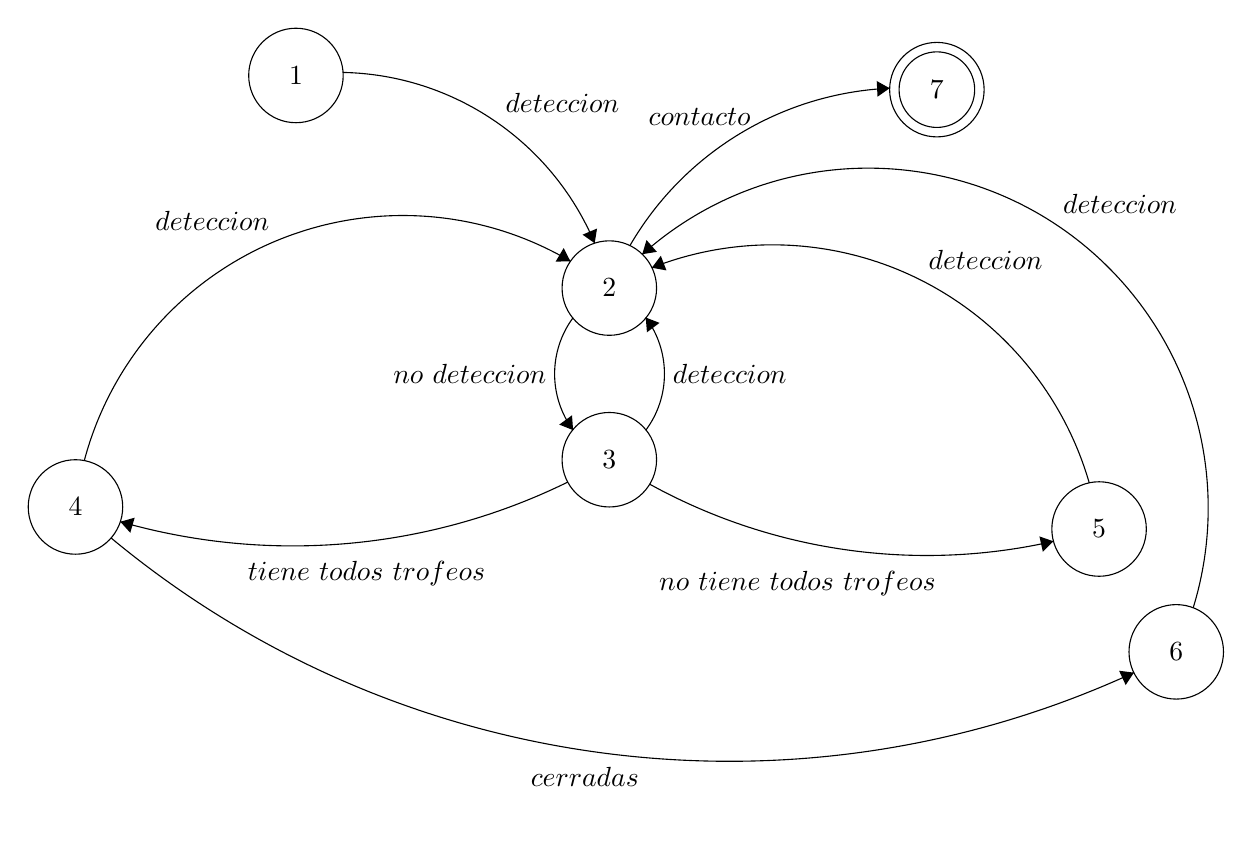
\begin{tikzpicture}[scale=0.2]
\tikzstyle{every node}+=[inner sep=0pt]
\draw [black] (18.5,-4.9) circle (3);
\draw (18.5,-4.9) node {$1$};
\draw [black] (38.4,-18.4) circle (3);
\draw (38.4,-18.4) node {$2$};
\draw [black] (38.4,-29.3) circle (3);
\draw (38.4,-29.3) node {$3$};
\draw [black] (4.5,-32.3) circle (3);
\draw (4.5,-32.3) node {$4$};
\draw [black] (69.5,-33.7) circle (3);
\draw (69.5,-33.7) node {$5$};
\draw [black] (74.4,-41.5) circle (3);
\draw (74.4,-41.5) node {$6$};
\draw [black] (59.2,-5.8) circle (3);
\draw (59.2,-5.8) node {$7$};
\draw [black] (59.2,-5.8) circle (2.4);
\draw [black] (21.49,-4.707) arc (88.84181:22.85288:17.734);
\fill [black] (37.47,-15.55) -- (37.62,-14.62) -- (36.7,-15.01);
\draw (35.42,-7.26) node [above] {$deteccion$};
\draw [black] (36.101,-27.421) arc (-143.55903:-216.44097:6.012);
\fill [black] (36.1,-27.42) -- (36.03,-26.48) -- (35.22,-27.07);
\draw (34.43,-23.85) node [left] {$no\mbox{ }deteccion$};
\draw [black] (40.71,-20.265) arc (36.73892:-36.73892:5.993);
\fill [black] (40.71,-20.27) -- (40.79,-21.21) -- (41.59,-20.61);
\draw (42.4,-23.85) node [right] {$deteccion$};
\draw [black] (35.759,-30.721) arc (-63.87939:-106.00611:39.678);
\fill [black] (7.35,-33.24) -- (7.98,-33.94) -- (8.26,-32.98);
\draw (22.98,-35.71) node [below] {$tiene\mbox{ }todos\mbox{ }trofeos$};
\draw [black] (66.605,-34.482) arc (-77.24077:-118.86465:36.441);
\fill [black] (66.6,-34.48) -- (65.71,-34.17) -- (65.93,-35.15);
\draw (50.34,-36.38) node [below] {$no\mbox{ }tiene\mbox{ }todos\mbox{ }trofeos$};
\draw [black] (71.707,-42.821) arc (-65.27917:-129.71678:61.433);
\fill [black] (71.71,-42.82) -- (70.77,-42.7) -- (71.19,-43.61);
\draw (36.84,-48.78) node [below] {$cerradas$};
\draw [black] (40.494,-16.255) arc (131.71542:-17.0893:21.578);
\fill [black] (40.49,-16.25) -- (41.42,-16.1) -- (40.76,-15.35);
\draw (70.83,-13.7) node [above] {$deteccion$};
\draw [black] (41.104,-17.106) arc (111.46121:16.14797:20.937);
\fill [black] (41.1,-17.11) -- (42.03,-17.28) -- (41.67,-16.35);
\draw (62.29,-17.28) node [above] {$deteccion$};
\draw [black] (5.06,-29.355) arc (165.12762:59.46253:20.937);
\fill [black] (35.93,-16.7) -- (35.5,-15.86) -- (34.99,-16.72);
\draw (13.19,-14.79) node [above] {$deteccion$};
\draw [black] (39.708,-15.703) arc (149.85656:92.55582:20.113);
\fill [black] (56.2,-5.71) -- (55.38,-5.25) -- (55.43,-6.25);
\draw (44.13,-8.1) node [above] {$contacto$};
\end{tikzpicture}
\end{center}

\begin{itemize}
	\item 1: Inicio, patrullar en unos puntos fijos.
	\item 2: Persecución.
	\item 3: Ir al último estado donde lo vio y patrullar ahí.
	\item 4: Ir a cerrar las puertas.
	\item 5: Ir a los últimos trofeos que quedan y patrullar ahí.
	\item 6: Ir a la salida y patrullar ahí.
	\item 7: Has tocado al Ladrón. Ganas la partida.
\end{itemize}

Nuestro agente es un agente con estados, de esta forma los perceptos pasados influyen en las acciones presentes (arriba se presenta un diagrama de estados que resume el comportamiento del agente). 
\texttt{Presentad una breve justificación de la arquitectura utilizada en cada uno de vuestros agentes (reactiva, deliberativa, híbrida, BDI, etc.), explicando las razones de vuestra elección.}
\section*{\large Sensores}
    \centering \includegraphics[width=0.4\textwidth]{vision.png}\\
\begin{itemize}
	\item Vista: el agente cuenta con un cono de visión que le permite ver a una cierta distancia de él con un cierto ángulo con respecto a la normal. No le permite en cambio, ver a través de las paredes.
	\item Oído: el agente cuenta con un radio de audición, aquello que suene dentro de esta región será percibido por el agente. Acompañamos esta habilidad sensórica del agente con la posibilidad de que el Ladrón haga ruído.
\end{itemize}

\texttt{Describid y justificad la elección de cada uno de los sensores que habéis decidido incluir, explicando su función y relevancia dentro del sistema.}
\section*{\large Actuadores}
\begin{itemize}
	\item Movimiento: el agente puede moverse bajo dos circunstancias, está dirigiendose a un punto de interés particular o esta patrullando. Naturalmente la cualidad de ``interes" de un punto es ignorada por el agente y para el siempre se esta dirigiendo a puntos igual de importantes.
	\item Tacto: el agente perseguirá al ladrón y cuando este lo suficiente lo tocará para ganar la partida.
\end{itemize}
\texttt{Describid y justificad la elección de cada uno de los actuadores que habéis decidido incluir, explicando su función y relevancia dentro del sistema.}
\end{document}
